\section{Praktische Anwendung der FM-Synthese}
\FloatBarrier
\subsection{Nachbildung eines Instruments}
Da es bei der FM-Synthese schwer fällt vorauszusagen, wie das durch die Synthese erzeugte Spektrum aussehen wird, ist es ein schwieriges Unterfangen mit dieser Technik ein echt wirkendes Instrument nachzubilden, beschrieben in \ref{PrinzipFM} - \nameref{PrinzipFM}.
Trotzdem gibt es einige Methoden den generierten Klang natürlicher wirken zu lassen. Diese werden im weiteren Verlauf dieses Kapitels vorgestellt und anschließend wird der Versuch unternommen den Klang eines Tones einer Querflöte nachzubilden.

\FloatBarrier
\subsubsection{Methoden zur Generierung eines Instrumententones mittels FM-Synthese}

Bei der Synthese eines Tones mittels FM-Synthese müssen zunächst die Parameter der Formel der FM-Synthese festgelegt werden. Hierzu kann das Frequenzspektrum und das Spektrogram des nachzubildenden Tones verwendet werden. Eine ausführliche Erklärung der einzelnen Parameter ist zu finden in Kapitel \ref{einfacheFM} - \nameref{einfacheFM}. 

Mit dem Offensichtlichstem kann gestartet werden, der Grundfrequenz. Sie ist im Normalfall die Frequenz mit dem größten Ausschlag im Spektrum. Sie kann als Trägerfrequenz $f_c$ verwendet werden. Der Abstand der Grundfrequenz zur ersten Seitenfrequenz und der Abstand der Seitenfrequenzen zueinander ist der zweite Anhaltspunkt. Dieser Abstand findet als Modulationsfrequenz $f_m$ Verwendung. Für harmonische Töne ist ein ganzzahliges Vielfaches der Grundfrequenz als Modulationsfrequenz nötig \cite[S. 528]{chowningPaper}. Der Modulationsindex $I$ kann mithilfe der Bessel Funktionen gefunden werden - siehe hierzu \ref{bulli:besselModIndexZusammenahang} - \nameref{bulli:besselModIndexZusammenahang}. Alternativ kann eine grobe Schätzung vorgenommen werden, hierzu ist die Faustformel Modulationsindex + 2 = Anzahl der sichtbaren Seitenfrequenzen nützlich. Sollte mittels der normalen FM-Synthese kein zufriedenstellendes Ergebnis erzielt werden können, sollte mit der komplexen FM-Synthese experimentiert werden. 

Bei der komplexen FM-Synthese finden mehrere Träger oder mehrere Modulatoren Verwendung. Diese können in Reihe oder parallel geschaltet werden. Außerdem kann auch die so genannte Feedback Frequenz Modulation genutzt werden, welche das voran gegangene Signal moduliert \cite[S. 399 f.]{hornerPaper}. Feedback-FM-Synthese kann außerdem eingesetzt werden um Rauschen zu erzeugen. Sie kann aber auch ein sehr komplexes Spektrum mit vielen Seitenfrequenzen erzeugen. Komplexe FM-Synthese findet Einsatz wenn mit der normalen FM-Synthese nicht ausreichend komplexe Spektren erzeugt werden können. Dies kann zum Beispiel der Fall sein wenn mehrere stetig fallende Seitenfrequenzen erzeugt werden sollen. Wenn bei einfacher FM-Synthese der Modulationsindex erhöht wird um mehr Seitenfrequenzen zu erzeugen, verändert sich die Stärke der Grundfrequenz, definiert durch die Bessel Funktionen - nachzulesen im Kapitel \ref{bulli:besselModIndexZusammenahang} - \nameref{bulli:besselModIndexZusammenahang}. Um dies zu vermeiden können die Modulatoren verschachtelt werden - nachzulesen im Kapitel \ref{cascade} - \nameref{cascade}

Eines der wichtigsten Grundbestandteile eines jeden Instrumententones ist die so genannte ADSR-Hüllkurve. Die Hüllkurve wird genutzt um die Amplitude des künstlich erzeugten Signals über den zeitlichen Verlauf festzulegen. ADSR steht für die einzelnen Phasen eines Tones: Attack, Decay, Sustain und Release. Diese Phasen sollen hier vereinfacht erklärt werden. Beim Drücken einer Taste wird der Ton angeschlagen und die Lautstärke des Tones steigt schnell bis zu einem maximalen Wert an. Diese Phase wird Attack genannt. Nachdem die maximale Lautstärke erreicht wurde, startet die Decay Phase. In dieser Phase sinkt die Lautstärke schnell auf einen geringeren Wert ab. Danach befindet sich der Ton in der Sustain Phase und die Lautstärke bleibt konstant oder fällt leicht ab, solange der Ton gespielt wird. Sobald die Taste losgelassen wird, befindet sich der Ton in der Release Phase und die Lautstärke nimmt wieder bis zu ihrem minimal Wert ab. In Abbildung \ref{fig:adsrDefault} ist der Verlauf der Lautstärke einer Standard ADSR-Hüllkurve noch einmal grafisch dargestellt.

\begin{figure} [ht]
\centering
  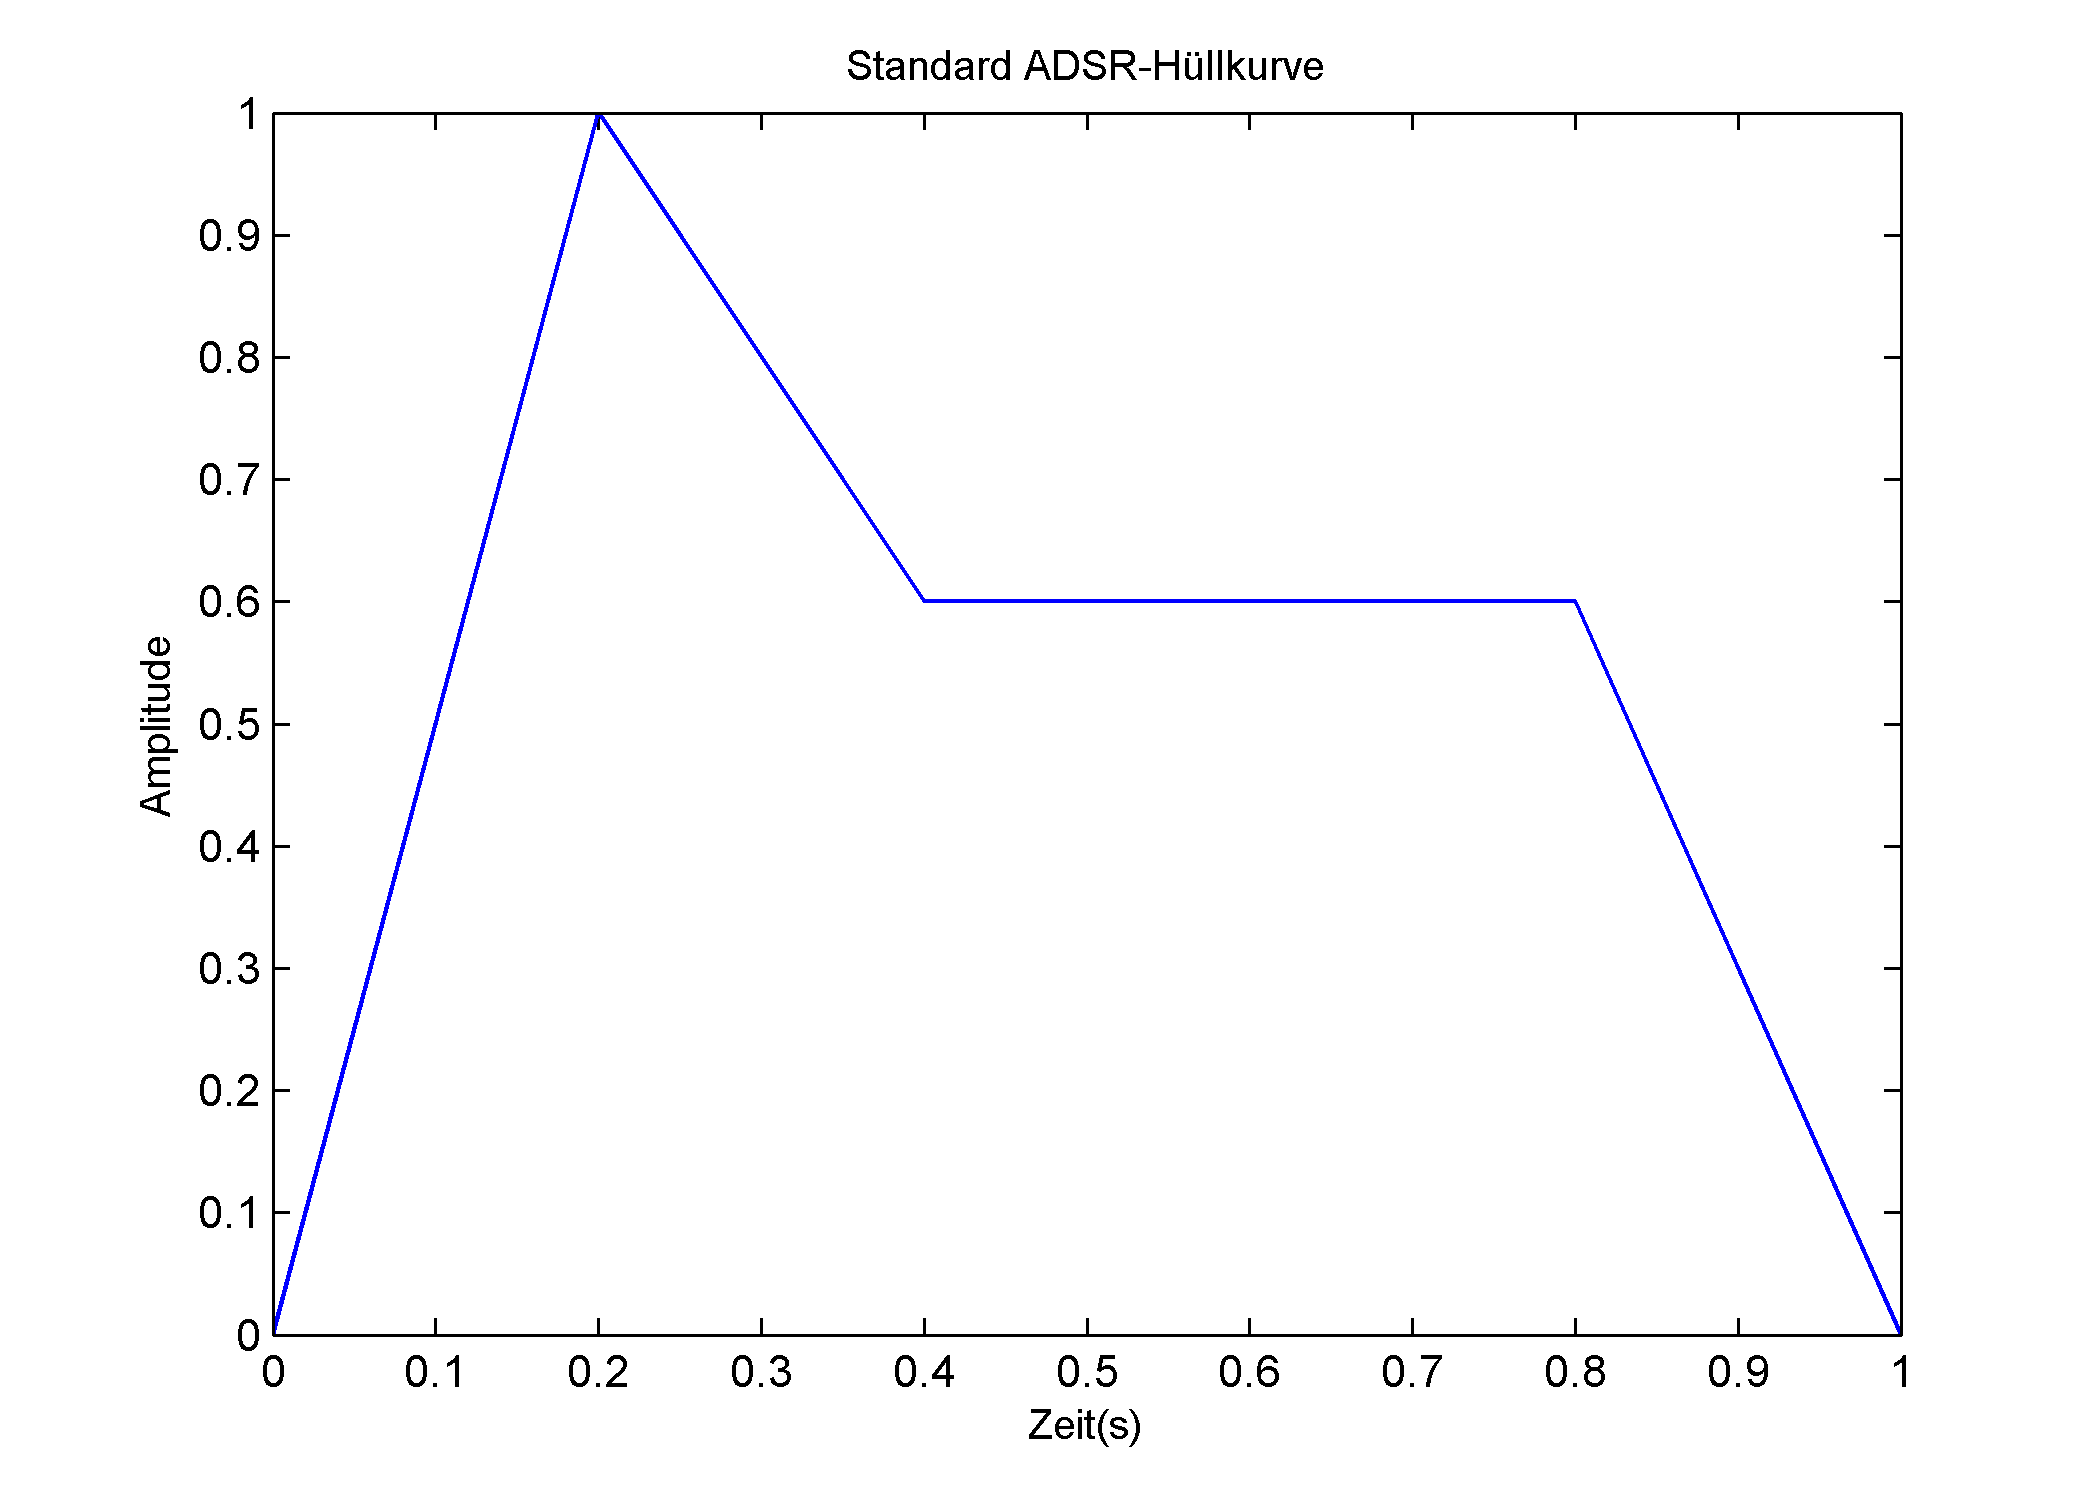
\includegraphics[width=0.5\textwidth]{adsrDefault.png}
\caption{Standard ADSR-Hüllkurve}
\label{fig:adsrDefault}
Quelle: Eigene Darstellung mit Matlab
\end{figure}

Da allerdings bei vielen Instrumenten die Lautstärke in den einzelnen Phasen der ADSR-Hüllkurve nicht gleichmäßig steigt oder sinkt, ist es nötig beliebig komplexe Kurven abbilden zu können. Bei vielen Instrumenten steigt beispielsweise die Lautstärke in der Attack Phase exponentiell an und fällt in der Decay und Release Phase auch wieder exponentiell ab. Manche Synthesizer bieten zusätzlich auch noch eine Hold Phase vor der Attack Phase, da es Instrumente gibt, die einige Zeit benötigen bis sie nach dem Anschlagen des Tones in die Attack Phase eintreten. In Abbildung \ref{fig:adsrTypical} wurden weitere für Instrumenten typische Hüllkurven dargestellt um zu verdeutlichen, dass die ADSR-Hüllkurve bei Instrumenten beliebig schlichte sowie komplexe Formen annehmen kann.

\begin{figure} [ht]
\centering
  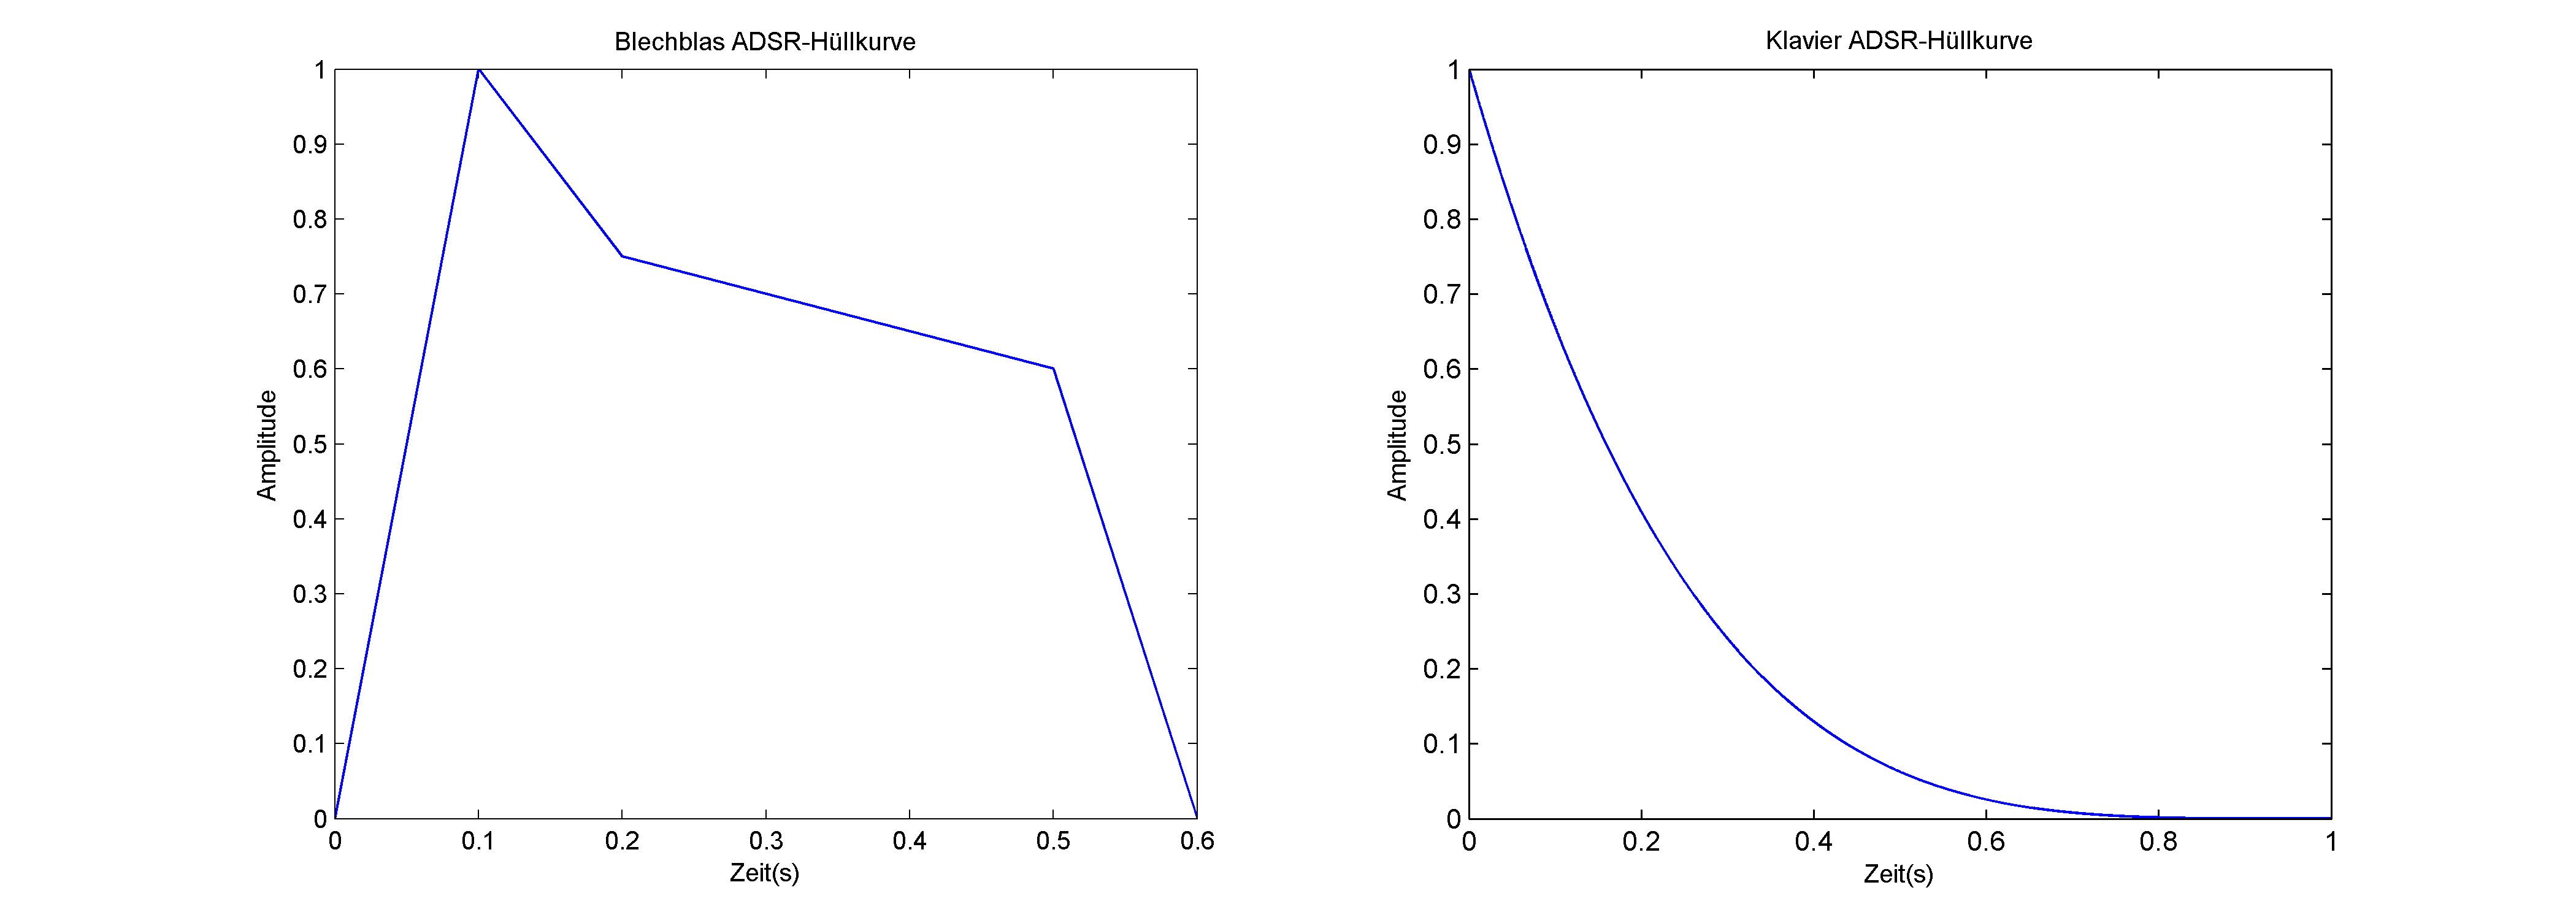
\includegraphics[width=1\textwidth]{adsrTypical.png}
\caption{Typische ADSR-Hüllkurve eines Blechblasinstrumentes und eines Klaviers}
\label{fig:adsrTypical}
Quelle: Eigene Darstellung mit Matlab
\end{figure}

Auch wenn das Hinzufügen einer ADSR-Hüllkurve den Klang des synthetisierten Tones schon natürlicher wirken lässt, hört sich der erzeugte Ton noch nicht wie ein echtes Instrument an. Eine weitere Möglichkeit ihn zu verbessern, stellt die Variierung des Modulationsindex über die Zeit oder die Amplitude dar. Somit kann die Anzahl der Seitenfrequenzen verändert werden, was zu einem lebendigeren Klang führt. Bei Blasinstrumenten beispielsweise, wird der Modulationsindex typischerweise über die Amplitude (also mit Hilfe der ADSR-Hüllkurve) variiert. \cite[S. 532]{chowningPaper}

Um den Klang des Tones noch weiter zu verbessern stellen Filter ein gutes Hilfsmittel dar. Filter können genutzt werden um das von der FM Synthese erzeugte Signal zu manipulieren. Dabei werden ungewollte Frequenzen gedämpft bzw. komplett herausgefiltert oder gewollte Frequenzen verstärkt. Typische Vertreter von Filtern sind Hochpassfilter, Tiefpassfilter, Bandpass und Bandsperre. \cite[S. 100-104]{stotz}

Das bisher erzeugte Signal ist noch ein reines Signal, welches so in der Natur nicht vorkommen kann. Bei Luft Verwirbelungen und Unebenheiten des Instrumentes tritt Rauschen auf. Dieses Rauschen trägt zum typischen Klangbild eines Instrumentes bei und sollte auch nachgebildet werden. Ein Rauschen kann mittels Feedback-FM-Synthese erzeugt werden, dafür muss der Modulationsindex der Feedback-FM-Synthese sehr hoch angesetzt werden. Das von der Feedback-FM-Synthese erzeugte Signal gleicht bei sehr hohem Modulationsindex einem weißen Rauschen. Anschließend kann dieses Rauschen mittels Multibandpassfilter um die jeweiligen ausgeprägten Frequenzen gefiltert werden. Würde das Rauschen nicht gefiltert werden, kann neben dem Ton, das Rauschen als solches wahrgenommen werden. [TODO CITE]

Um den Klang des synthetisierten Tones noch natürlicher zu gestalten, könnte dem Ton zusätzlich ein Hall-Effekt hinzugefügt werden.


\FloatBarrier
\subsubsection{Nachbildung eines Tones einer Querflöte mittels FM-Synthese}

Im Laufe dieses Kapitels soll ein Ton einer Querflöte mittels FM-Synthese erzeugt und mit den oben beschriebenen Techniken verfeinert werden. Alle Beispiele sind in Matlab erstellt und können mit den beiliegenden Source-Code nachgestellt werden. In Abbildung \ref{fig:plotFluteOrig} sind Spektrogram, Waveform und Spektrum des originalen Querflöten Tones abgebildet. Mit den Informationen aus den vorliegenden Grafiken wird versucht, diesen spezifischen Ton nachzubilden.

\begin{figure} [h!t!b!]
\centering
  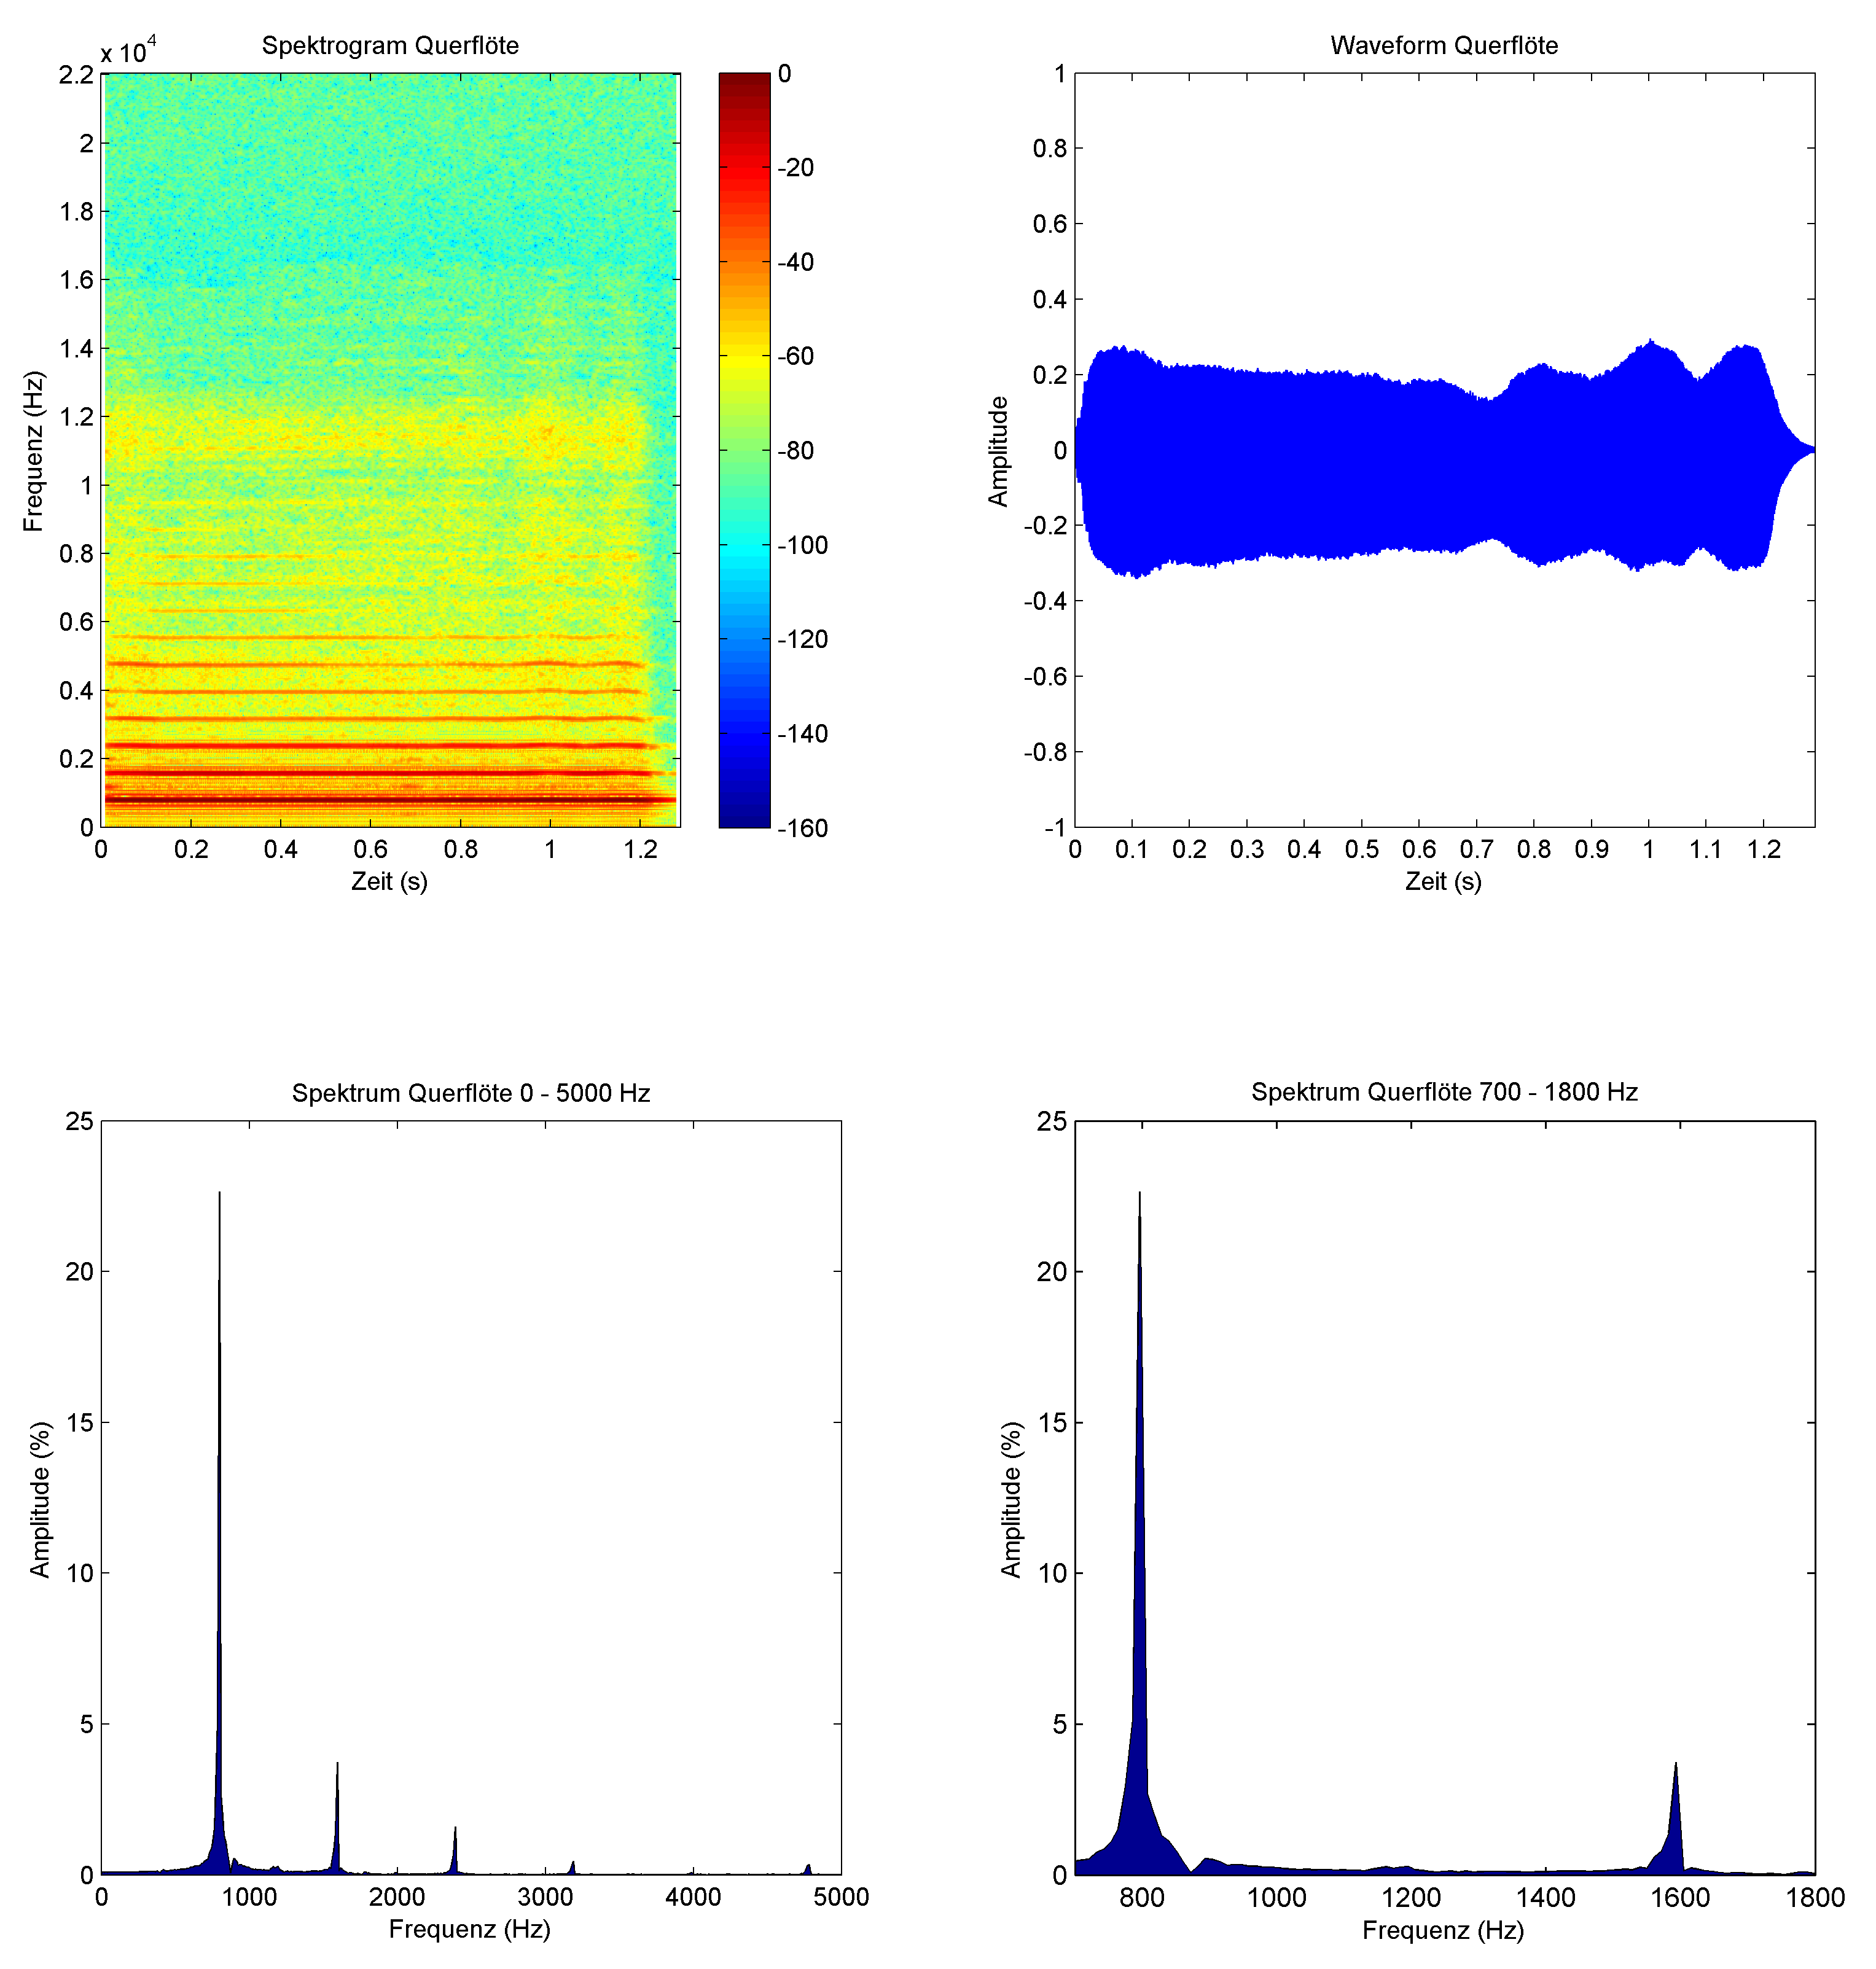
\includegraphics[width=1\textwidth]{plotFluteOrig.png}
\caption{Plot des Spektrograms, der Waveform und des Spektrums eines echten Tones einer Querflöte}
\label{fig:plotFluteOrig}
Quelle: Eigene Darstellung mit Matlab
\end{figure}

Anhand des Spektrums können bereits einige Erkenntnisse für die FM-Synthese ausgelesen werden. Zunächst ist zu bemerken, dass die am stärksten ausgeprägte Frequenz bei etwa 800 Hz liegt. Bei genauerer Betrachtung wird sichtbar, dass die Frequenz nicht exakt bei 800 Hz sondern bei 796.75 Hz ihren maximalen Ausschlag erreicht. Dies entspricht am ehesten einem G5 mit 784 Hz \cite[S. 181]{borucki}. Diese Frequenz (796.75 Hz) werden wir bei der FM-Synthese als Trägerfrequenz nutzen. Im Spektrum sind außerdem noch mehrere Seitenfrequenzen zu erkennen. Die erste dieser Seitenfrequenzen befindet sich bei etwa dem doppelten der Grundfrequenz. Bei genauerer Betrachtung wird sichtbar, dass sie ihren maximalen Amplitudenwert wirklich genau bei dem doppeltem der Grundfrequenz (1593.5 Hz) hat. Also ist der Abstand zwischen Grundfrequenz und erster Seitenfrequenz genauso groß wie die Grundfrequenz. Hierbei ist zu bemerken, dass der Abstand von einem ganzzahligen Multiplikator mit der Grundfrequenz typisch für einen harmonischen Ton ist \cite[S. 528]{chowningPaper}. Die nächsten Seitenfrequenzen haben jeweils wieder denselben Abstand von 796.75 Hz zur jeweiligen vorangegangenen Seitenfrequenz. Aus dieser Beobachtung können wir unsere Modulationsfrequenz von 796.75 Hz schließen. Anhand der Anzahl der sichtbaren Seitenfrequenzen im Spektrum können wir eine ungefähre Abschätzung unseres Modulationsindexes wagen. Somit wird als Modulationsindex für die ersten Tests vorerst 0.5 angenommen. 

\begin{figure} [ht]
\centering
  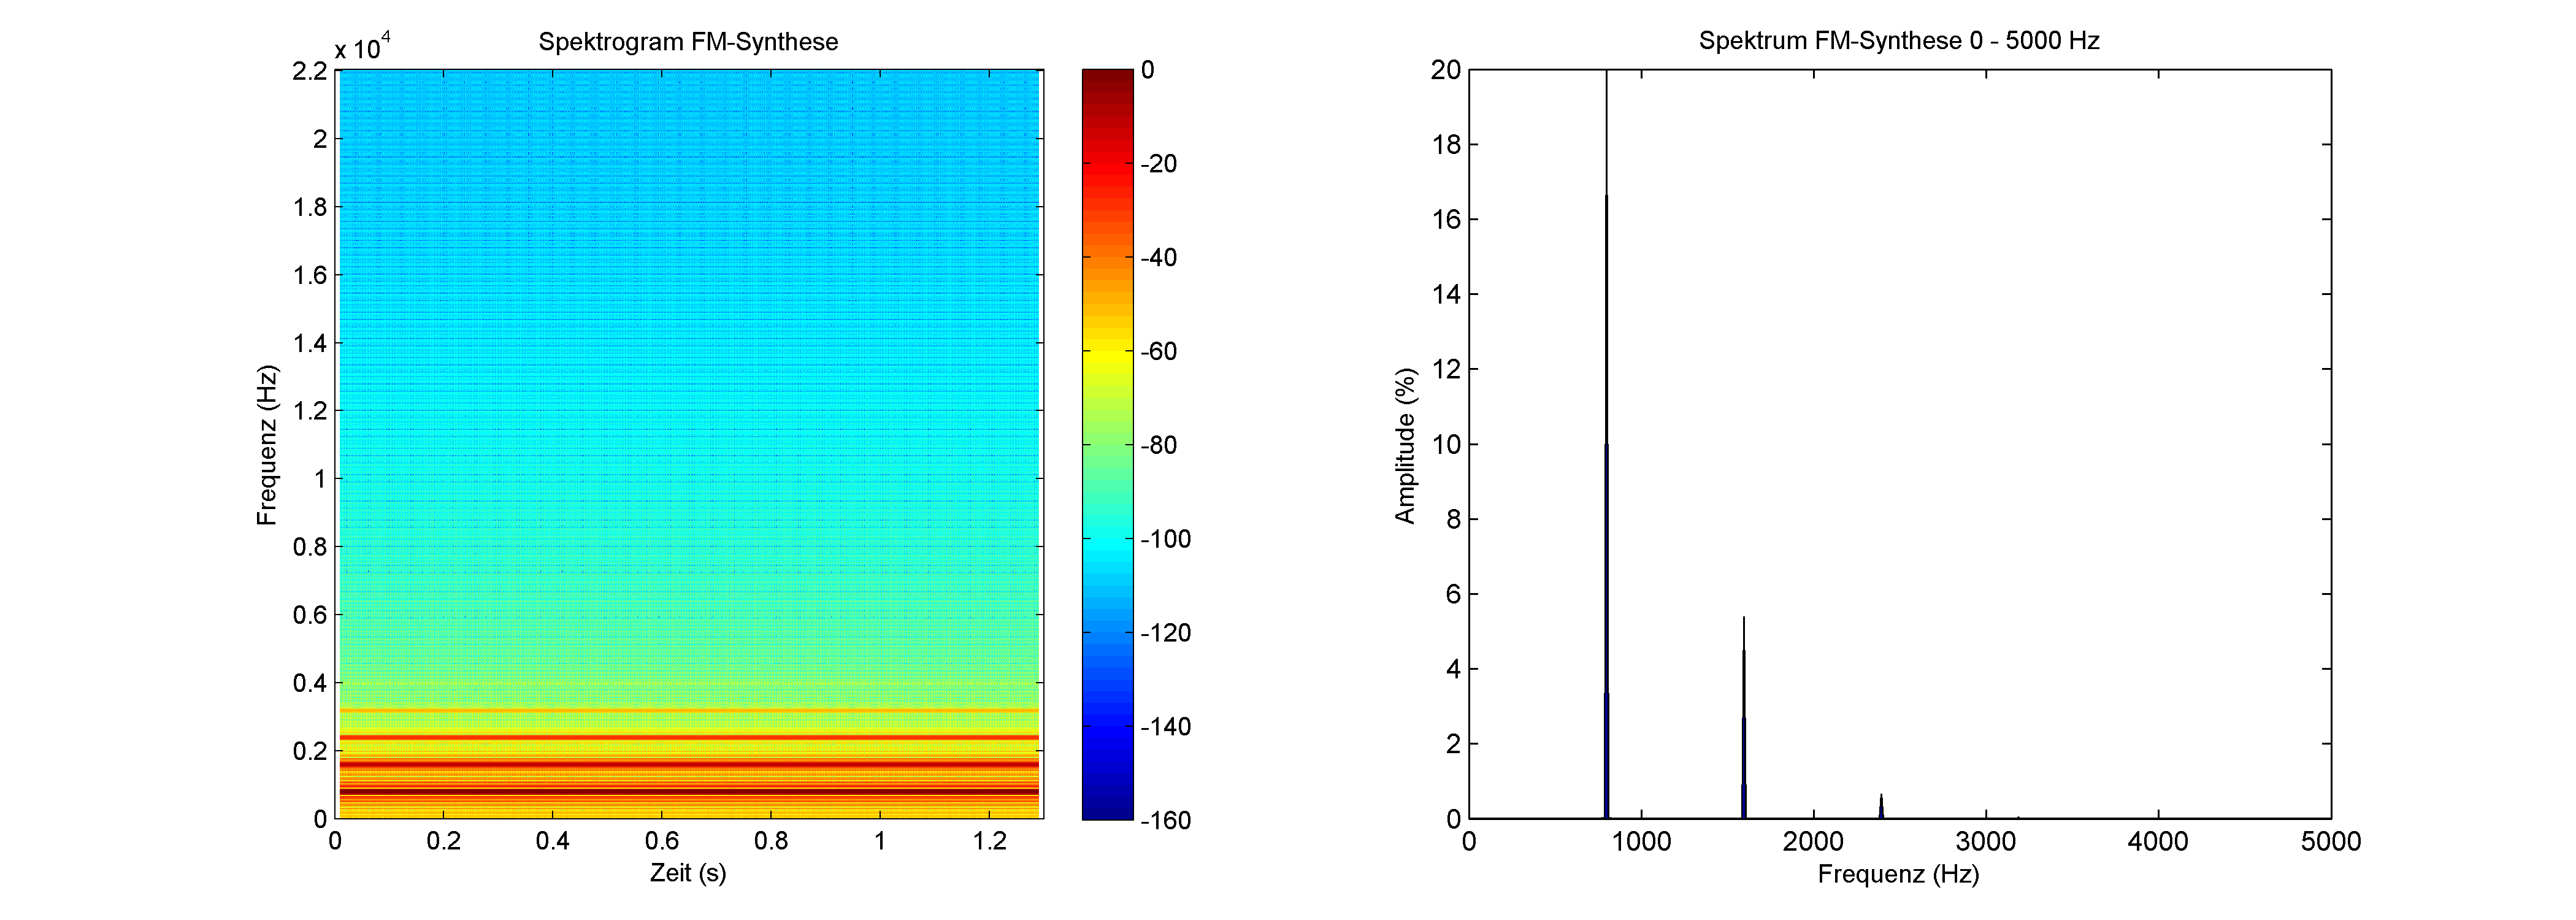
\includegraphics[width=1\textwidth]{plotFMSyntheseI05.png}
\caption{Plot des Spektrograms und des Spektrums der FM-Synthese mit den Parametern $f_c = 796.75 Hz$, $f_m = f_c$ und $I = 0.5$ }
\label{fig:plotFMSyntheseI05}
Quelle: Eigene Darstellung mit Matlab
\end{figure}

Ein erstes Spektrum der FM-Synthese mit den eben festgelegten Werten kann in Abbildung \ref{fig:plotFMSyntheseI05} begutachtet werden. Beim Evaluieren der Ergebnisse dieses Spektrums fällt auf, dass die erste Seitenfrequenz im Verhältnis zur Grundfrequenz einen viel stärkeren Ausschlag aufweist als es bei der Querflöte der Fall ist. Außerdem fällt danach die Amplitude der 2. und 3. Seitenfrequenz viel stärker ab als bei dem Instrument. Sieht man sich jetzt noch das Spektrogram (ebenfalls in Abbildung \ref{fig:plotFMSyntheseI05}) an, fällt im Vergleich zum Spektrogram der Querflöte die sehr viel geringer Anzahl an Seitenfrequenzen auf. Die Seitenfrequenzen bei 4000 Hz und darüber sind bei dem Instrument noch deutlich sichtbar während sie bei der FM-Synthese schon bei 4000 Hz kaum noch existent sind. Versucht man jetzt den Modulationsindex zu erhöhen um die Anzahl der Seitenfrequenzen zu erhöhen, verlagert sich die Amplitude unserer Trägerfrequenz auf die Seitenfrequenzen, damit werden die Seitenfrequenz stärker und die Träger Frequenz schwächer, zu sehen in Abbildung \ref{fig:spektrumFMSyntheseI2}. 

\begin{figure} [ht]
\centering
  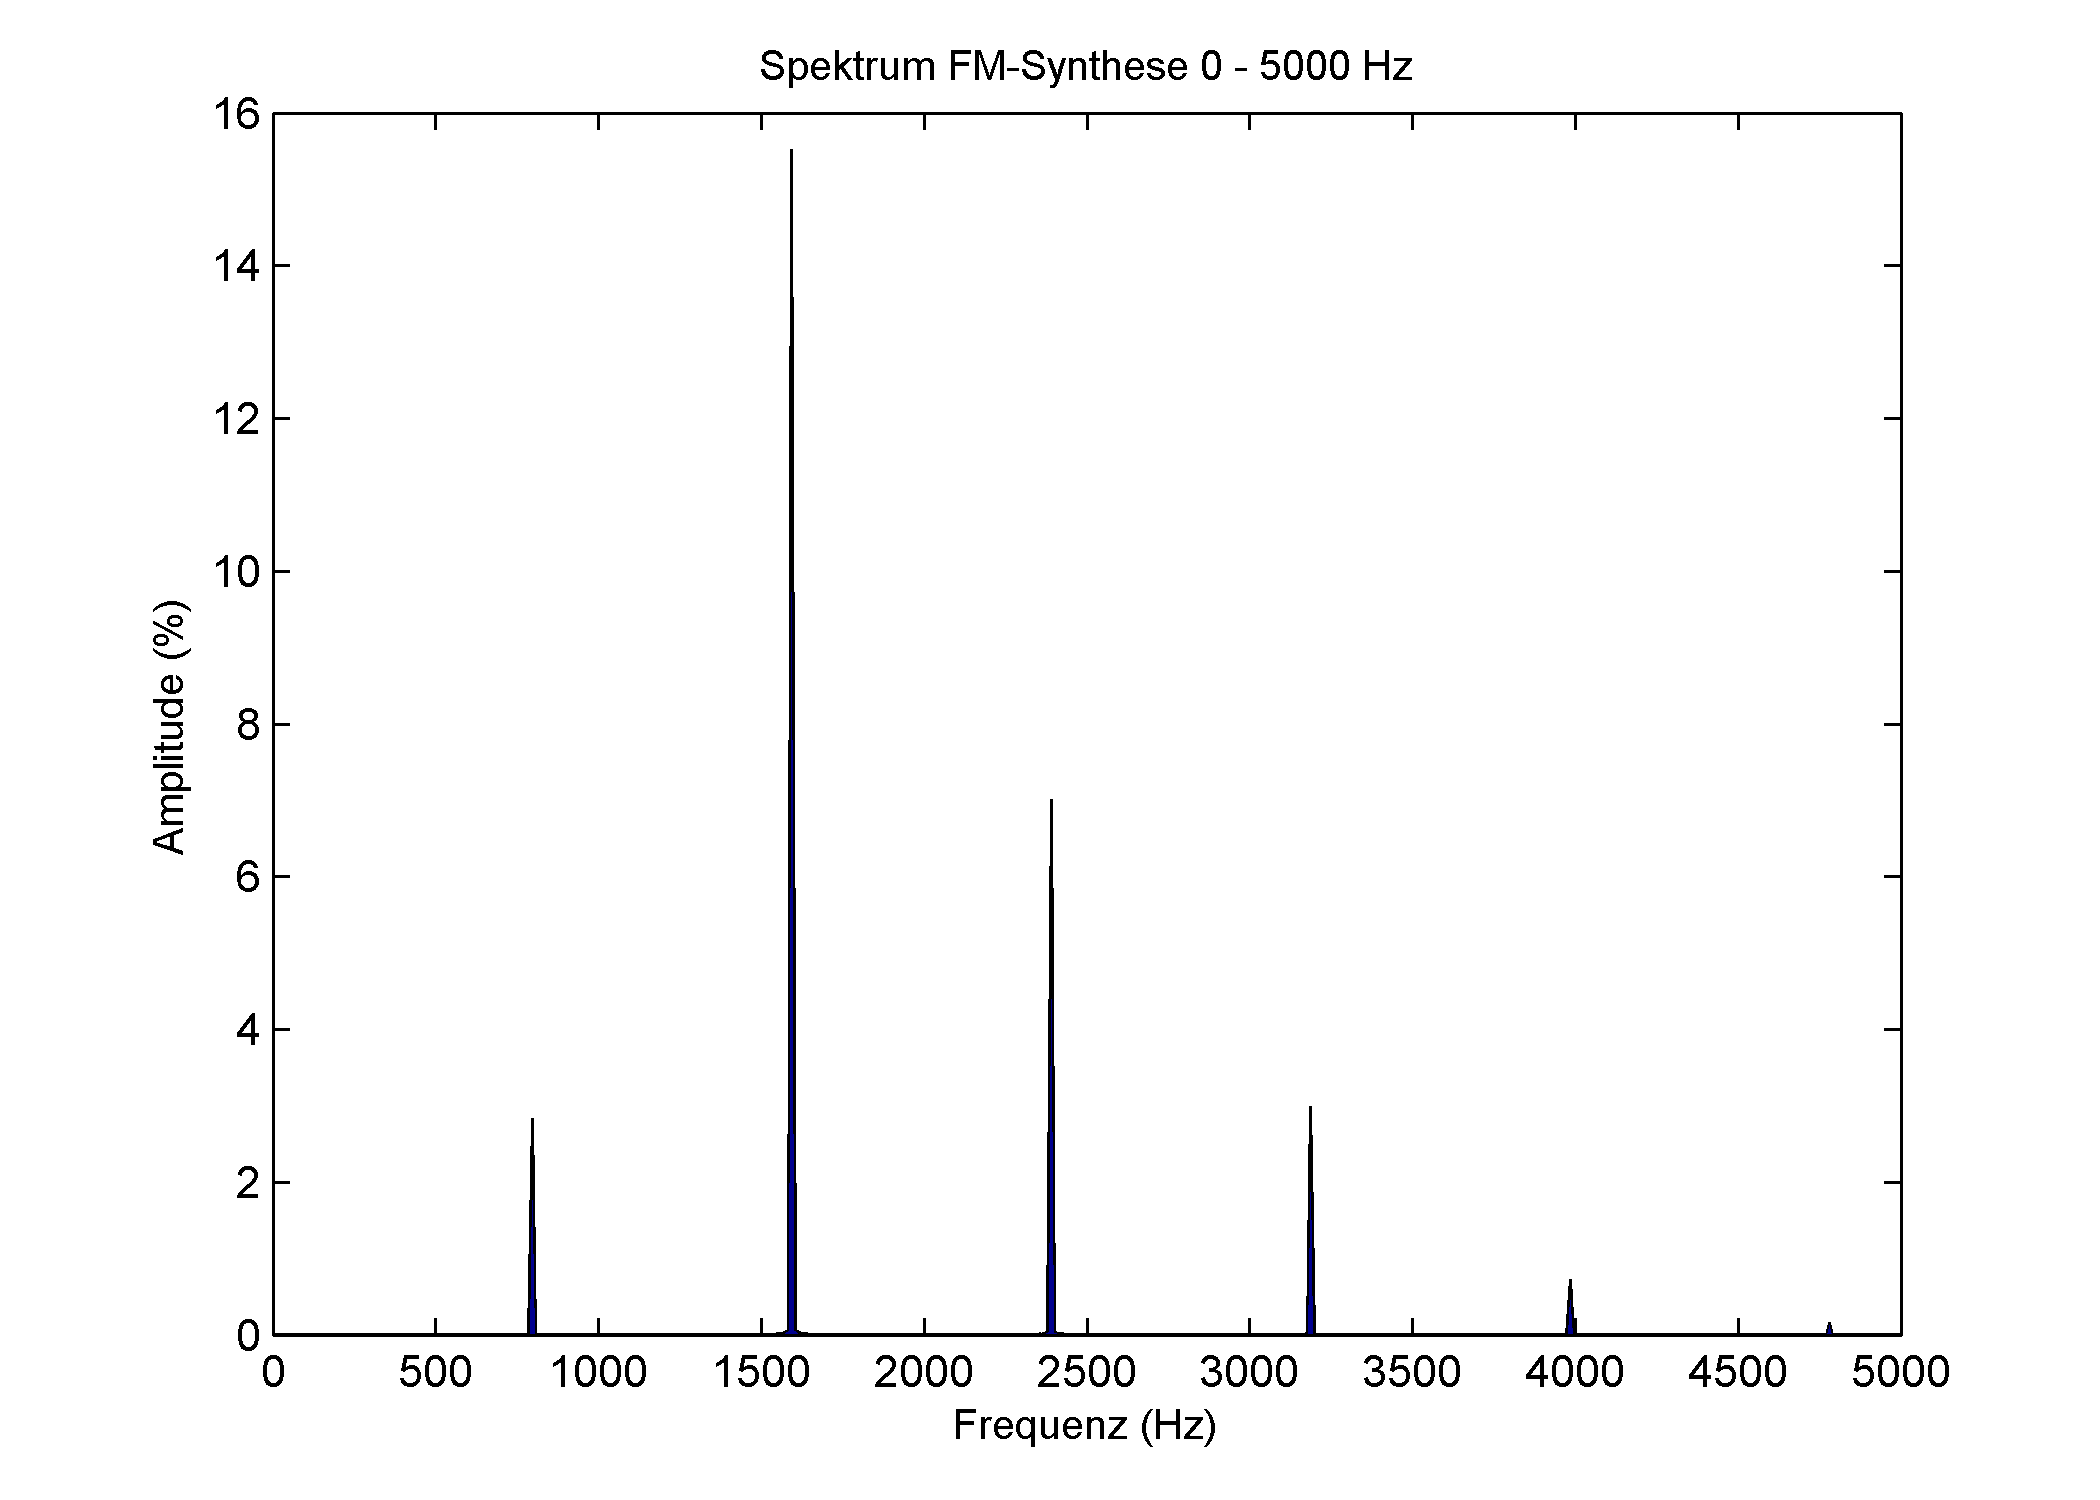
\includegraphics[width=0.5\textwidth]{spektrumFMSyntheseI2.png}
\caption{Plot des Spektrums der FM-Synthese mit den Parametern $f_c = 796.75 Hz$, $f_m = f_c$ und $I = 2$}
\label{fig:spektrumFMSyntheseI2}
Quelle: Eigene Darstellung mit Matlab
\end{figure}

Um dieses Verhalten zu umgehen müssen wir uns der komplexen FM-Synthese widmen. Hier werden mehrere Modulatoren verschachtelt um eine größere Anzahl an Seitenfrequenzen zu erzeugen. Allerdings ist es bei der komplexen FM-Synthese nochmal schwerer im Vergleich zur einfachen FM-Synthese, wie stark die Amplituden der einzelnen Seitenfrequenzen ausgeprägt sind, deshalb braucht es hier einige Experimente um auf das gewünschte Ergebnis zu erzeugen. In Abbildung \ref{fig:plotFMSyntheseKomplex4Mod} kann das Ergebnis der FM-Synthese mit 4 Modulatoren betrachtet werden. Dieses Spektrum ähnelt dem der Querflöte schon sehr viel stärker und auch das Spektrogram weißt in den Intensitäten der Seitenfrequenzen eine deutliche Ähnlichkeit auf.

\begin{figure} [ht]
\centering
  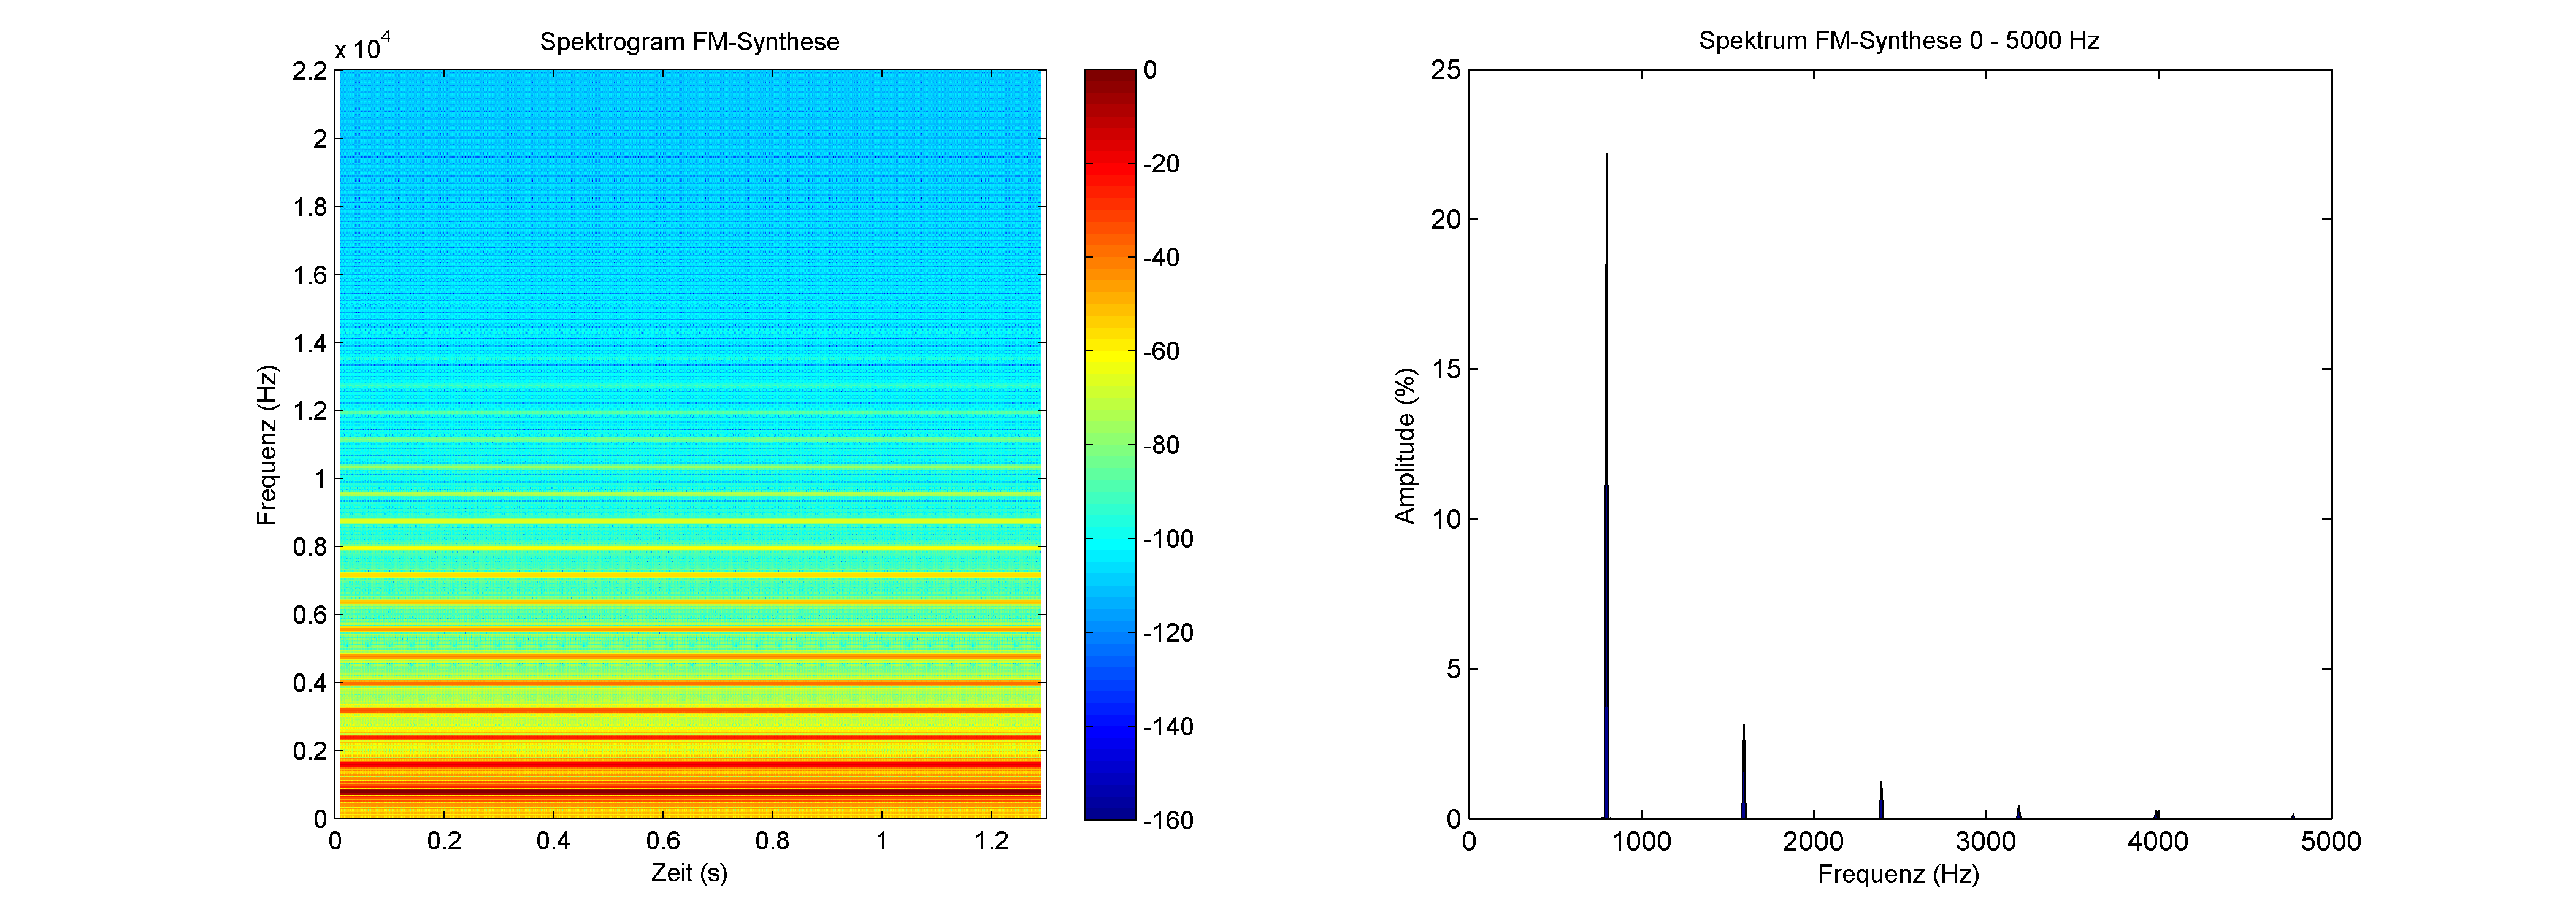
\includegraphics[width=1\textwidth]{plotFMSyntheseKomplex4Mod.png}
\caption{Plot des Spektrograms und des Spektrums der FM-Synthese mit 4 Modulatoren und den Parametern $f_c = 796.75 Hz$, $f_m1 = f_m2 = f_m3 = f_m4 = f_c$, $I_1 = 0.3$, $I_2 = 0.5$, $I_3 = 1$ und $I_4 = 1$}
\label{fig:plotFMSyntheseKomplex4Mod}
Quelle: Eigene Darstellung mit Matlab
\end{figure}

Da die Grundeinstellung der FM-Synthese mit den oben genannten Parametern ein zufriedenstellendes Signal erzeugt, können wir uns jetzt der Veredlung des Tones widmen. Zuerst wird dem Signal ein Vibrato hinzugefügt. Durch das Hinzufügen des Vibratos, schwingt der erzeugte Ton leicht und wirkt lebendiger und nicht ganz so künstlich. Dies kann bewerkstelligt werden indem die Modulationsfrequenz leicht erhöht oder verringert wird. Auch hierbei muss experimentiert werden, welche Erhöhung der Modulationsfrequenz das gewünschte Ergebnis erzeugt. Als sehr ähnlich zum Original Ton hat sich in diesem Fall eine Erhöhung um 2.5 Hz herausgestellt. Unsere neue Modulationsfrequenz ist somit $f_m = f_c + 2.5$. In Abbildung \ref{fig:spektrumFMSyntheseVibrato} wird die Auswirkung des Vibratos sichtbar, es bilden sich um die Seitenfrequenzen weitere recht gering ausgeprägte Frequenzausschläge.

\begin{figure} [ht]
\centering
  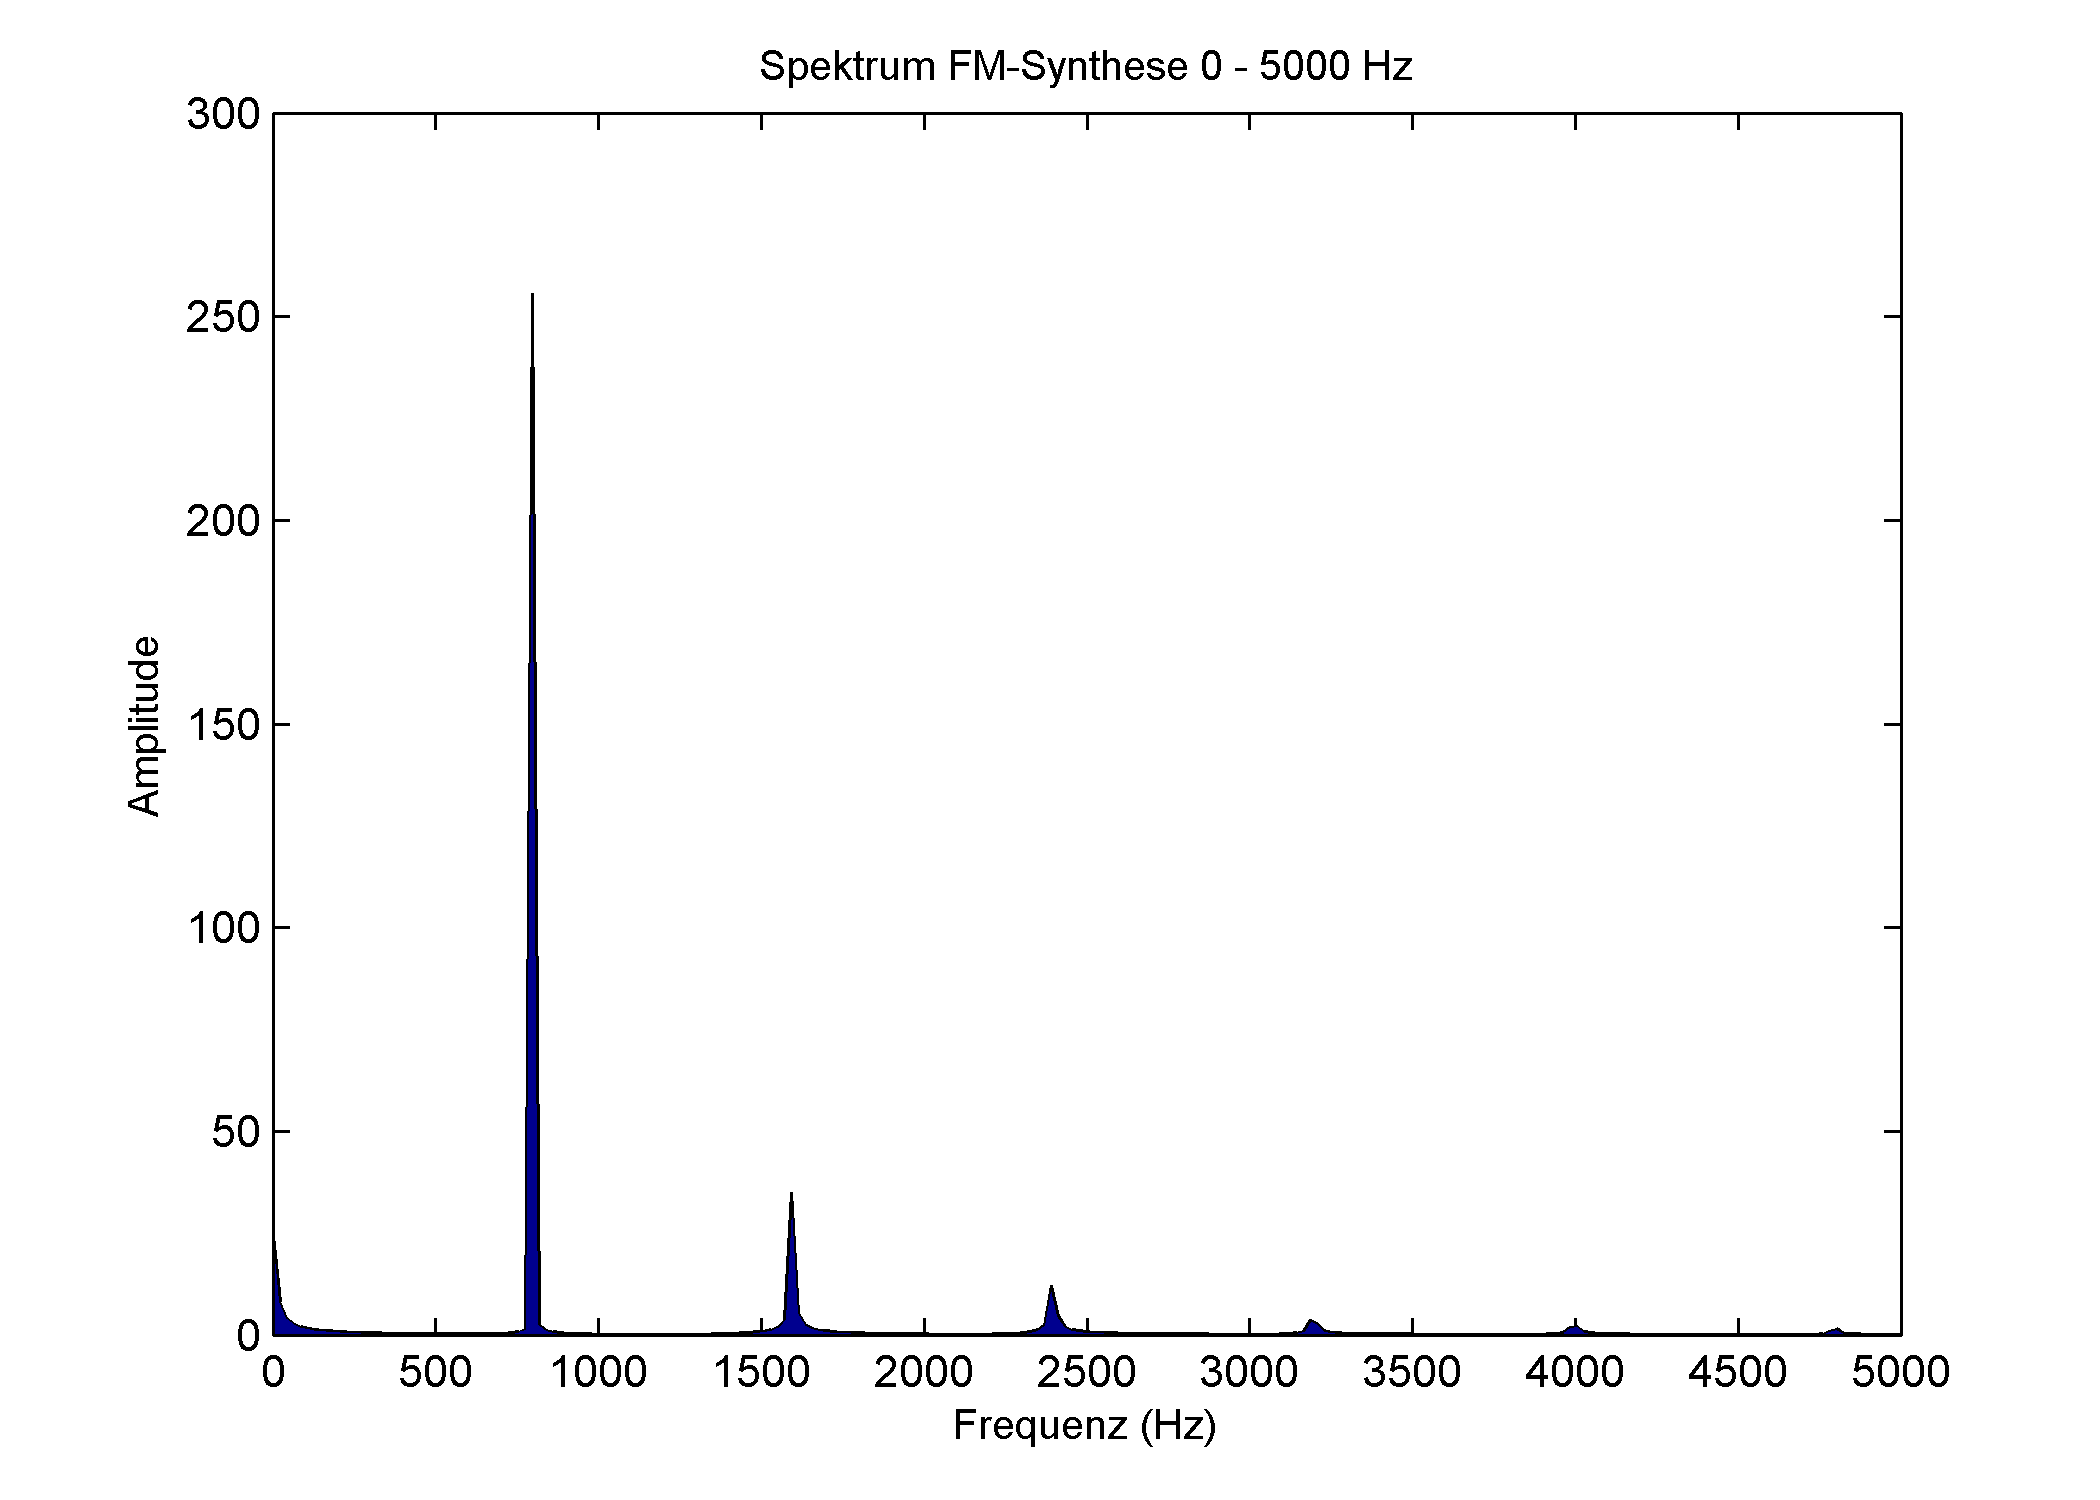
\includegraphics[width=0.5\textwidth]{spektrumFMSyntheseVibrato.png}
\caption{Plot des Spektrums der FM-Synthese mit 4 Modulatoren, Vibrato und den Parameter $f_c = 796.75 Hz$, $f_m1 = f_m2 = f_m3 = f_m4 = f_c + 2.5$, $I_1 = 0.3$, $I_2 = 0.5$, $I_3 = 1$ und $I_4 = 1$}
\label{fig:spektrumFMSyntheseVibrato}
Quelle: Eigene Darstellung mit Matlab
\end{figure}

Der nächste wichtige und einfach hinzuzufügende Bestandteil des synthetisierten Tones ist die ADSR-Hüllkurve. Um generell eine Querflöte nachzuahmen wäre eine Hüllkurve wie in Abbildung \ref{fig:adsrFlute} (links) gezeigt möglich. Allerdings versuchen wir den originalen Ton der Querflöte so gut wie möglich nachzuahmen, hierfür wurde eine komplexere Hüllkurve nach dem Beispiel der Waveform des originalen Tones generiert. Bei dieser Hüllkurve wurde Attack, Decay und Release von der allgemeinen Hüllkurve übernommen und die Sustain Phase angepasst, zu sehen in Abbildung \ref{fig:adsrFlute} (rechts). 

\begin{figure} [ht]
\centering
  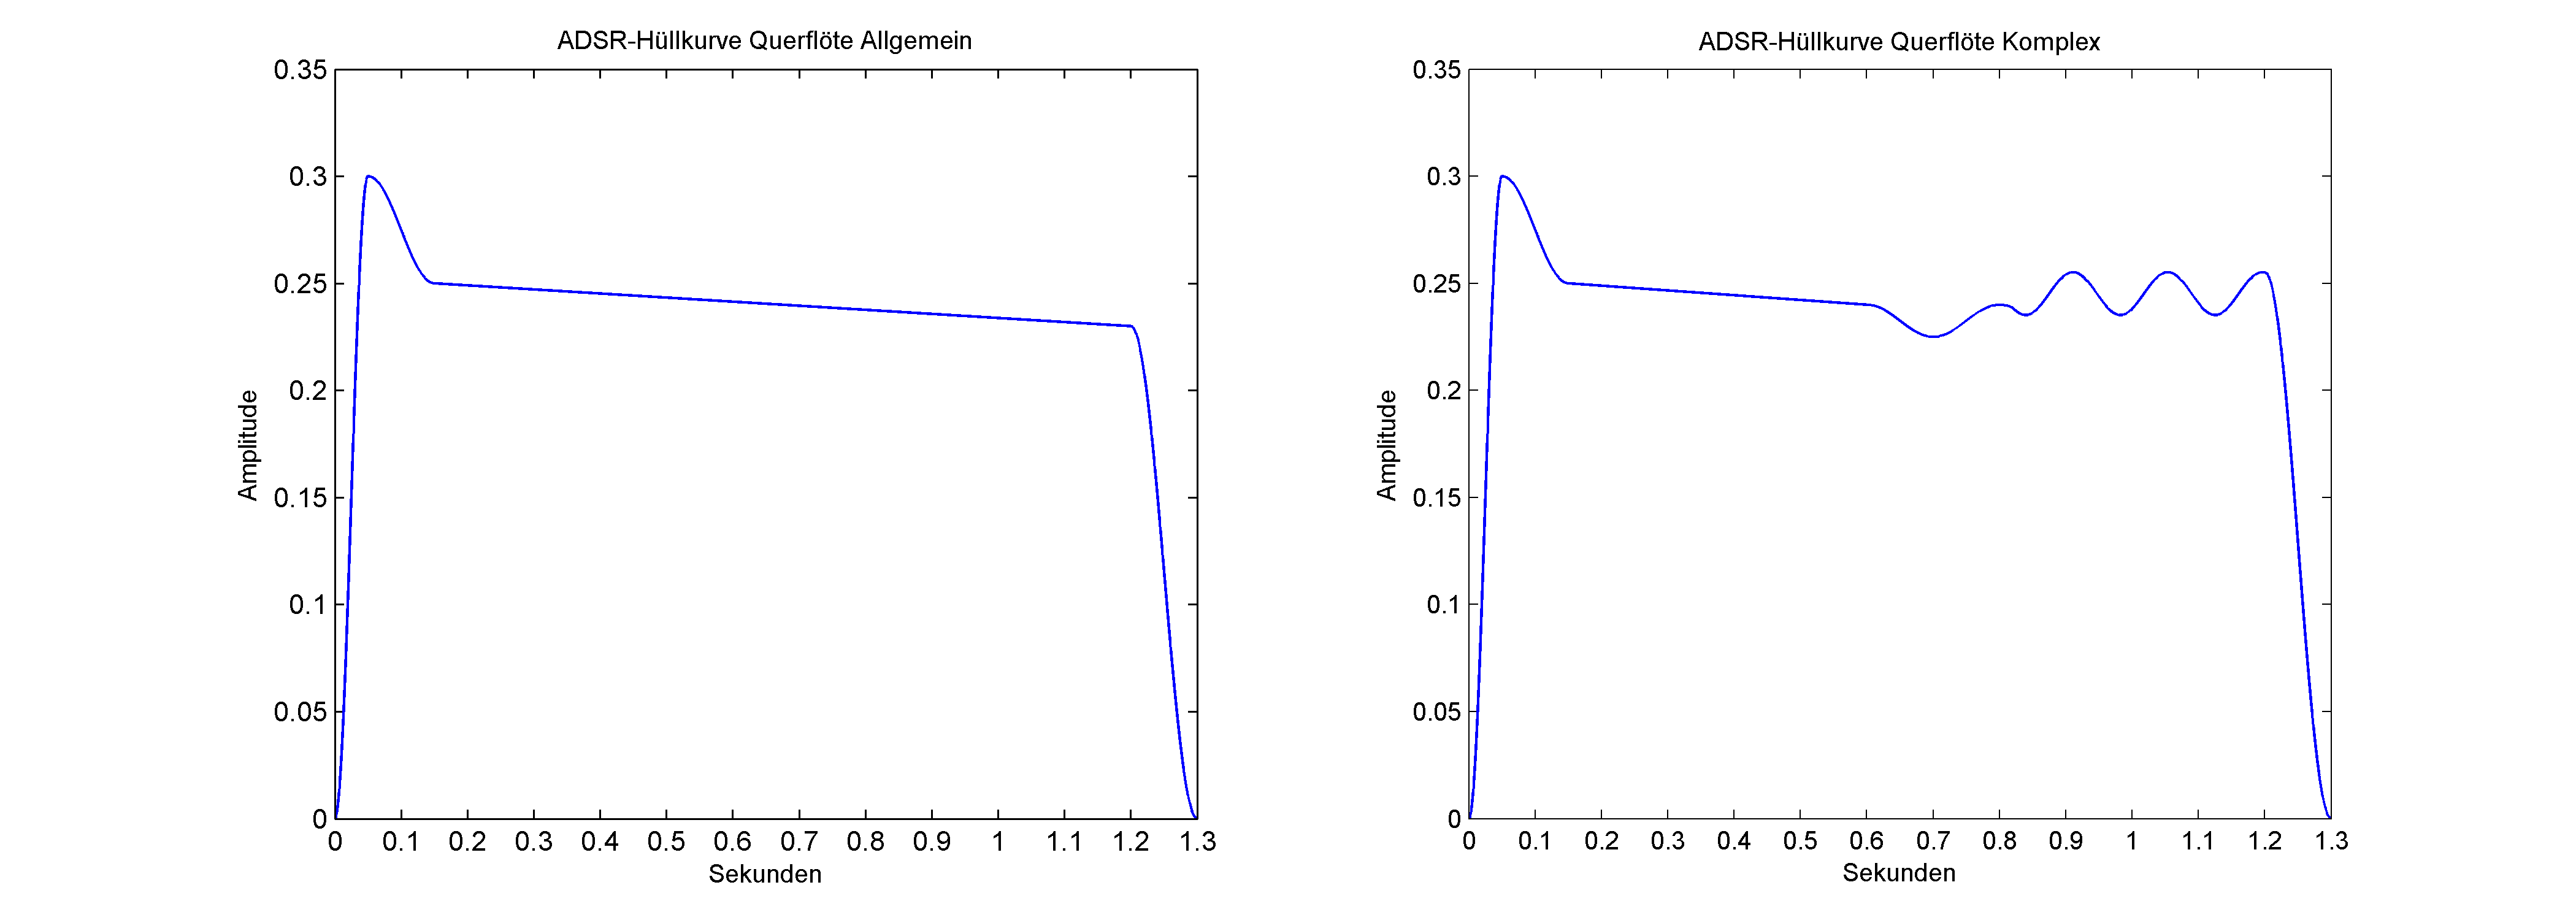
\includegraphics[width=1\textwidth]{adsrFlute.png}
\caption{Plot der ADSR-Hüllkurve einer Querflöte und der hier genutzten, komplexeren Hüllkurve}
\label{fig:adsrFlute}
Quelle: Eigene Darstellung mit Matlab
\end{figure}

Nach Hinzufügen der ADSR-Hüllkurve, fällt im Spektrogram auf, dass die Seitenfrequenzen trotz geringerer Amplitude bei Attack und Release Phase einen größeren Ausschlag als beim Instrument aufweist. Dieser Ausschlag kann verringert werden, indem der erste Modulationsindex mit der ADSR-Hüllkurve variiert wird. 

Nachdem Vibrato, Variabler Modulationsindex und ADSR-Hüllkurve hinzugefügt wurden, hat sich das Spektrogram zur Abbildung \ref{fig:plotFMSyntheseKomplex4Mod} kaum geändert. Es wird nur der Vibrato durch die etwas breiteren Seitenfrequenzen und die ADSR-Hüllkurve durch Ansteigen des Spektrums zu Beginn des Tones und Abfallen des Spektrums nach 1.2 Sekunden sichtbar. Der Ton hört sich von der Tonhöhe und der Intensität schon stark nach dem originalen Querflötenton an. Allerdings fehlen noch die typischen Blas- und Luft Verwirbelungsgeräusche sowie das sehr dominante Anblasgeräusch. Um die typischen Blasgeräusche zu erzeugen wird zunächst ein Rauschen mittels Feedback-FM-Synthese mit hohem Modulationsindex erzeugt. Würde das Rauschen ohne weitere Arbeitsschritte dem synthetisierten Signal hinzugefügt, könnte das Rauschen stark herausgehört werden. Um dies zu verhindern muss das Rauschen vorerst gefiltert werden. Hierzu wird ein Multibandpassfilter über alle möglichen Seitenfrequenzen erstellt. Das gefilterte Rauschen wird anschließend noch mit einer ADSR-Hüllkurve veredelt. Dieser Schritt ist nötig, da während der Attack Phase des original Tones, wie im Spektrogram in Abbildung \ref{fig:plotFluteOrig} zu sehen, das Rauschen durch das Anblasen des Instrumentes sehr scharf heraus sticht. Zusätzlich kann noch ein sehr leises Rauschen der Feedback-FM-Synthese ohne Filter über das ganze Frequenzspektrum gelegt werden um auch in den höheren Frequenzen einen leichten Ausschlag im Spektrogram kenntlich zu machen. Trotz des verstärkten Rauschens zu Beginn des Tones, fehlt noch der das stark hörbare Anblasgeräusch. Beim Betrachten des Spektrums und des Spektrograms fallen noch zwei recht starke Ausschläge zu Beginn des Signals auf. Ein Ausschlag befindet sich bei 904.3 Hz und der Zweite bei 1182 Hz. Beide Frequenzen können mit einem einfachen Sinus erzeugt und mit einer ADSR-Hüllkurve, die nur eine kurze Attack Phase aufweist und danach komplett abfällt, modelliert und zum Signal addiert werden. In Abbildung \ref{fig:spektrogramFMSyntheseComplete} ist das Ergebnis der FM-Synthese mit den, in diesem Kapitel, besprochenen Veredelungen gezeigt. In den Plots sind die Ähnlichkeiten zum originalen Ton deutlich zu sehen.

\begin{figure} [h!t!b!]
\centering
  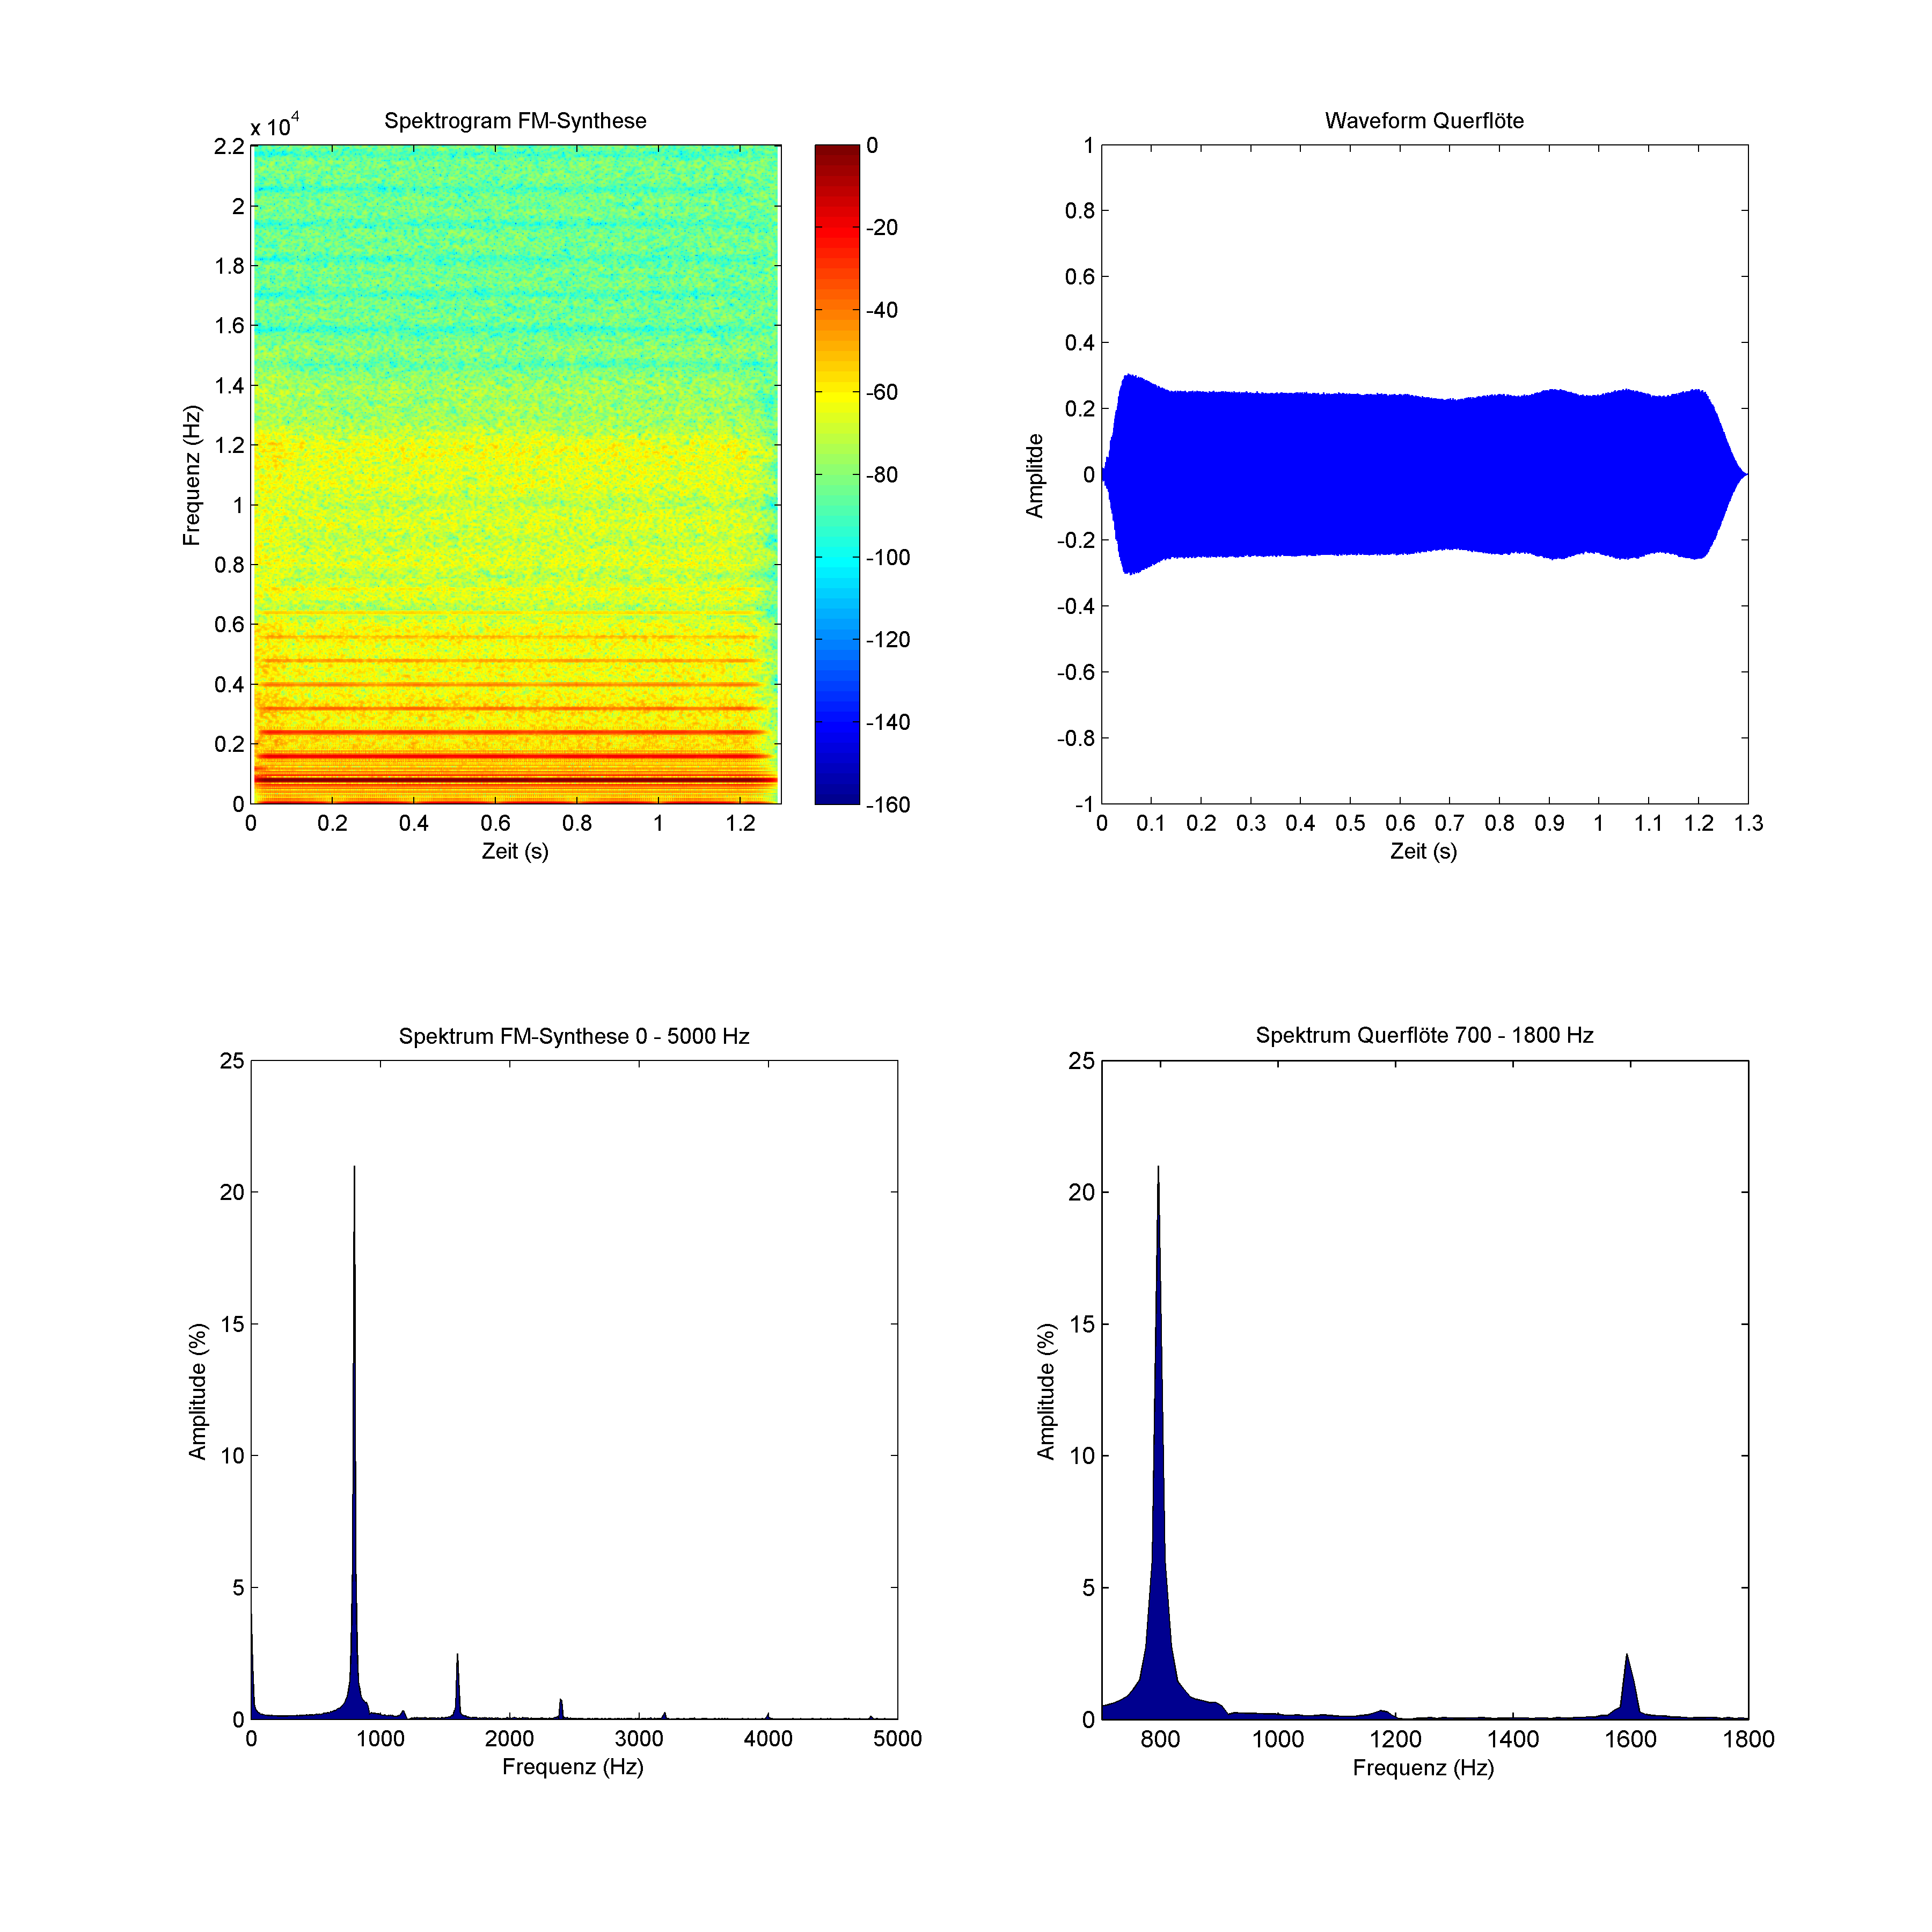
\includegraphics[width=1\textwidth]{spektrogramFMSyntheseComplete.png}
\caption{Plot des fertigen Tones der FM-Synthese mit 4 Modulatoren, ADSR-Hüllkurve, Variablem Modulationsindex, Vibrato, Rauschen und Anblasgeräusch}
\label{fig:spektrogramFMSyntheseComplete}
Quelle: Eigene Darstellung mit Matlab
\end{figure}

Der in diesem Kapitel synthetisierte Ton nähert sich dem originalen Flötenton sehr gut. Trotzdem weißt der Flötenton noch etwas mehr Lebendigkeit auf, da das gesamte Signal nicht so statisch wie das der FM-Synthese wirkt. Dieses Ergebnis zeigt, dass es sehr wohl möglich ist, wenn auch mit erheblichem Aufwand verbunden, mit der FM-Synthese einen natürlich wirkenden Instrumententon zu erzeugen. Gerade in diesem Beispiel fällt allerdings auf das der synthetisierte Ton im Vergleich zum originalen Ton nicht ganz so lebendig empfunden wird. Das hängt in diesem Fall vor allem an der Spielweise des Querflötenspielers.


\FloatBarrier
\subsubsection{FM Parametrisierung mittels genetischer Algorithmen}

Mittels genetischer Algorithmen ist es möglich Parameter der FM-Synthese zu ermitteln, die nötig sind um einen Ton zu erzeugen, der einem echten Instrument nachempfunden ist. Diese Algorithmen teilen einen echten Ton eines Instrumentes mittels Schneller Fourier Transformation in seine einzelnen Frequenzen auf und versuchen verschiedene Parameter für die Synthese aus. Das entstandene Signal wird wieder mittels Schneller Fourier Transformation aufgeteilt und die so gewonnenen Ergebnisse verglichen. Mit diesem Verfahren können recht zuverlässig realistisch synthetisierte Töne erzeugt werden, die von einem originalen Instrument kaum zu unterscheiden sind. Eine ausführliche Erklärung der FM Parametrisierung mittels Genetischer Algorithmen kann in Andrew Horners Artikel ''Nested Modulator and Feedback FM Matching of Instrument Tones'' nachgelesen werden.

\FloatBarrier
\subsection{Implementierung eines FM-Synthesizers zur Demonstration der Synthese Parameter}

Zu Beginn dieser Arbeit wurde zum besseren Verständnis der FM-Synthese ein kleiner Software Synthesizer in C++ mit der Hilfe des JUCE Frameworks geschrieben. Das JUCE Framework wurde hierfür ausgewählt, da es gerade für ein Audioprogramm gut geeignet ist. Es bietet bereits Funktionen zur Ausgabe eines Audio Signals und Möglichkeiten zur Erstellung einer Benutzeroberfläche. Zudem ist das JUCE Framework Cross Plattform fähig.

Zunächst wurde eine einfache FM-Synthesizer Klasse geschrieben und diese an das Audio Ausgabesystem des JUCE Frameworks angebunden. Dabei ruft die Soundkarte eine Methode des Programms auf und erwartet, dass der übergebene Puffer mit Audiodaten gefüllt wird. Das Programm füllt den gegebenen Puffer mit Daten die mit der FM-Synthesizer Klasse generiert wurden. Später wurde das Programm dann noch um die visuelle Darstellung des erzeugten Audiosignals erweitert. Außerdem ist es möglich dem FM-Synthesizer einen Hüllkurvengenerator zu übergeben, welcher bei der Erzeugung des Audiosignals den Amplitudenwert für die einzelnen Samples bereitstellt. Die Amplitudenwerte werden ebenfalls visuell dargestellt.

Da gerade die Änderung der Parameter und das jeweils resultierende Klangbild zum Verständnis hilfreich sind, wurden Möglichkeiten in das Programm eingebaut um sowohl den Modulationsindex als auch die Modulationsfrequenz sowie die Oktave zu ändern. Das Ändern der Parameter ist mittels einfachem Tastendruck möglich. Zusätzlich wurde das Programm so angepasst, dass es mittels Tastendruck verschiedene Töne gespielt werden können. Die Tasten ''C'', ''D'', ''E'', ''F'', ''G'', ''A'' und ''B'' entsprechen dabei jeweils ihrem tonalen Äquivalent. Beim Drücken der Taste startet die Hüllkurve in die Attack Phase, geht dann über in die Decay und schließlich in die Sustain Phase. Wird die Taste losgelassen startet die Release Phase und der Ton klingt ab. Mit den Tasten ''1'' und ''2'' kann der Modulationsindex inkrementiert sowie dekrementiert werden. Um die Modulationsfrequenz zu ändern können die Pfeil hoch und Pfeil runter Tasten genutzt werden. Die Octave lässt sich mit den Tasten ''+'' und ''-'' verändern.

Das entstandene Programm bietet eine gute Möglichkeit die Parameter der FM-Synthese während der Wiedergabe eines Tones zu verändern und hilft so zu verstehen was beim Ändern dieser passiert. Natürlich ist das entstandene Programm nicht so flexibel und mächtig wie beispielsweise das Programm FM8 von Native Instruments. Trotzdem bietet es einen einfachen Einstieg in die FM-Synthese, somit wurde das Ziel der Programmierung des Tools erreicht.
\FloatBarrier
